\chapter{Freemind Example}
\label{ch:Freemind Example}

The example used for this paper is the \textit{automatic save file} feature of Freemind, also used in the paper \emph{A Survey of Feature Location Techniques} by \textit{Julia Rubin} and \textit{Marsha Chechik} \cite{rubin2013survey}. Freemind is an open source  mind-mapping tool. The \textit{automatic save file} feature is a good example, because of it's name. Parts of the name are also mentioned in other features, which makes it slightly more difficult to only locate this specific feature.
A related callgraph of the important parts is shown in Fig 2.1.

\begin{wrapfigure}{r}{0.5\textwidth}
  \centering
  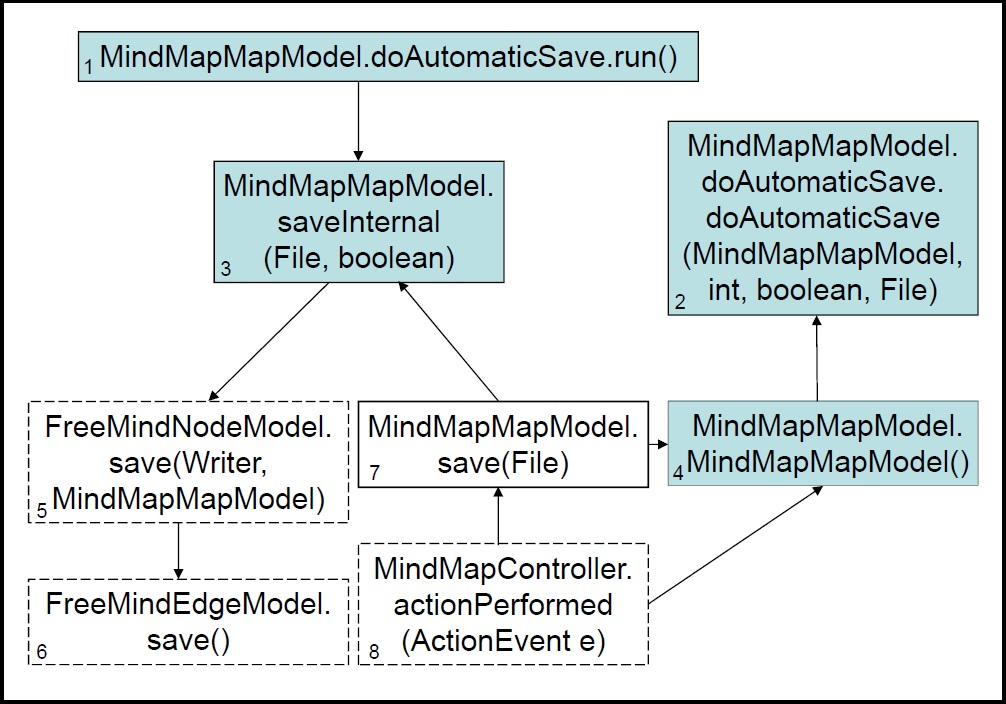
\includegraphics[width=\linewidth]{src/pic/freemind_callgraph}
  \caption{The Freemind callgraph \cite{FrM16} \cite{rubin2013survey}}
  \label{pic:freemind callgraph}
\end{wrapfigure}

In the graph only the relevant constructors and methods are shown and numbered with indices from 1 to 8. These will be further referenced by using the number sign \# and then the corresponding number. Also the feature of the regarded function are highlighted with a blue background colour. These are the methods which should be located if the \emph{automatic save file} function is the wanted feature. Note that all the methods of different classes can in addition call other methods and constructors, which are irrelevant to the feature.
So as it is shown within the graph the feature is mainly implemented by two methods of a subclass of \emph{MindMapMapModel} so called \emph{doAutomaticSave}:
\begin{itemize} 
\item the constructor, which is \#2. This constructor gets a few parameters to configure the \emph{doAutomaticSave}-function and registers the class in the scheduling queue, so that it gets called.
\item the \emph{run()}-function \#1. This Methods gets called after the class is registered in the scheduling queue and everytime a special event occurs. That can be different, like a period of time to schedule an automatic save or a preset number of actions within the main-program. It calls the \emph{saveInternal}-method to do the actual \textit{save}-operation.
\end{itemize}

\newpage
Regarding the previously mentioned definition of a feature by Rajlich and Chen in \autoref{Rajlich_Chen}, the regarded feature can be defined as the following: \newline
\begin{tabular}{ l  l }
  name & \emph{automatic save file}  \\
  intension & saves a file automatically after the occurring of an event\\
 extension & \#1,  \#2, \#3 and \#4\\
\end{tabular}
The methods \#5 to \#8 are not in the extension of the \emph{automaticSaveFile} feature.
Mainly \# 5 and \#6 are called by methods of the \emph{automaticSaveFile} feature, but are not relevant to the specifies of this function.
\#7 and \#8 in fact call \#3 and \#4, but they handle a user triggered save-event, which obviously is not important to the \emph{automaticSaveFile} feature.
\newline \newline
While all feature location techniques try to achieve the same goal, which is locating the matching feature extension to a given feature intension, they differ in the underlying base of assumptions they make to be able to get the traceability. It will be declared more specific in chapter~\ref{ch:Classification and Methodology}. 
